% !TEX root = /Users/Gela/Desktop/Thesis_latex/thesis.tex

\section{Flowchart investigation}
\label{Flowchart}
To obtain a system to run tests on some different flowchart are considered. The current pump will be replaced by two pumps. Following requirements will be desirable when obtaining a updated model of the flowchart:

\begin{itemize}
\renewcommand\labelitemi{ }
\item Pressure drop over the membrane is high
\item Flow through membrane is high
\end{itemize}
\textbf{The model shall contribute with the following:}
\begin{itemize}
\renewcommand\labelitemi{ }
\item Permeate conductivity (minimized)
\item Fouling on the membrane (minimized)
\item Temperature dependencies 
\item Waste water going through drain (minimized)
\end{itemize}

\textbf{Mainly two different systems containing two pumps were considered:}

\subsection{System 1}
The first system with one with pump on feed side and one pump on permeate side, as seen in Figure \ref{fig:FlowCInves1}. This setup contributes with the ability to create a net pressure over the membrane with a low, or even a under pressure on permeate side, whilst the feed pressure pump

\begin{figure}[h]
    \centering
    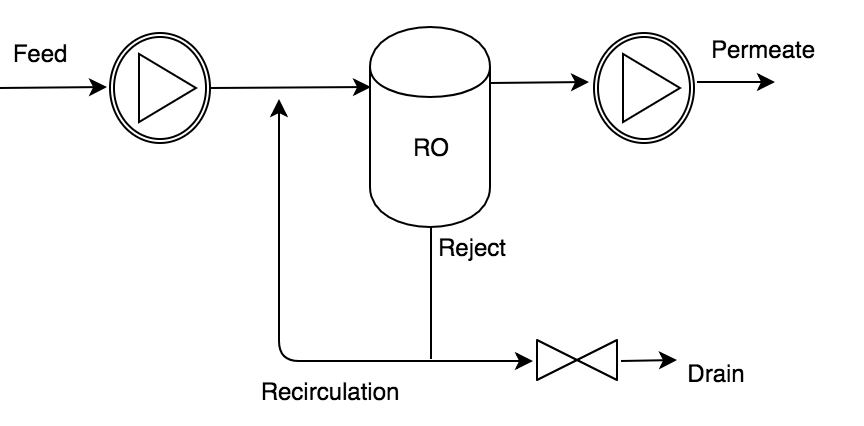
\includegraphics[width=0.4\textwidth]{FlowCInves1}
    \caption{System 1}
    \label{fig:FlowCInves1}
\end{figure}

\subsection{System 2}
The second system considered with one pump on feed side and one pump on rejectside, in recirculation path, seen in Figure \ref{fig:Sys2}.
\begin{figure}[h]
    \centering
    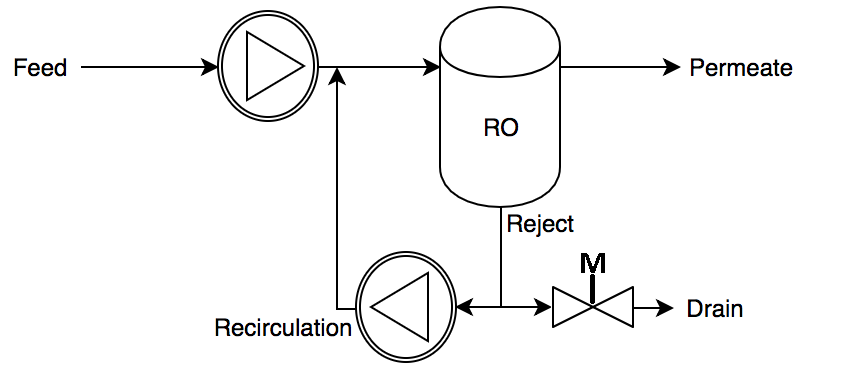
\includegraphics[width=0.4\textwidth]{Sys2}
    \caption{System 2}
    \label{fig:Sys2}
\end{figure}

\section{Tests}
In order to compare results of the current system, furthermore called "Current System" and the updated system, some test will be done on the current setup. Reasonable values were investigated in order to meet requirements of the Water device. Same points will be tested on the comparing system to evaluate any improvements on the membrane performance. Points to investigate can be seen in Table \ref{tab:testcases}:\\
\begin{table}[h]
\begin{tabular}{ |p{1cm}||p{3cm}|p{4cm}|}
 \hline
 \textbf{Case}&Temperature $^\circ$C& Feed Conductivity (\SI{}{\micro\siemens}) \\
 \hline
 1 & 18 $^\circ$C  & 280 \SI{}{\micro\siemens}  \\
 2   &  18 $^\circ$C  & 500 \SI{}{\micro\siemens}  \\
 3 &  18 $^\circ$C & 1000 \SI{}{\micro\siemens}  \\
 4 &18 $^\circ$C& 2000 \SI{}{\micro\siemens}\\
 5   &18 $^\circ$C& 3000 \SI{}{\micro\siemens}\\
 \hline
 6 & 30 $^\circ$C & 280 \SI{}{\micro\siemens}\\
 7 & 30 $^\circ$C & 500 \SI{}{\micro\siemens}\\
 8 & 30 $^\circ$C& 1000 \SI{}{\micro\siemens}\\
 9 & 30 $^\circ$C& 2000 \SI{}{\micro\siemens}\\
 10 & 30 $^\circ$C& 3000 \SI{}{\micro\siemens}\\
 \hline
 11 & 40 $^\circ$C& 280 \SI{}{\micro\siemens}\\
 12 & 40 $^\circ$C& 500 \SI{}{\micro\siemens}\\
 13 & 40 $^\circ$C & 1000 \SI{}{\micro\siemens}\\
 14 & 40 $^\circ$C& 2000 \SI{}{\micro\siemens}\\
 15 & 40$^\circ$C & 3000 \SI{}{\micro\siemens}\\
\hline
\end{tabular}
\caption{Testcases}
    \label{tab:testcases} 
\end{table}


\section{Modeling}
Simscape software tool described in section \ref{Simscape} is used to do a physical modeling in order to achieve the characteristics of the membrane. Mathematical equations from the manufacturer of the membrane and physics of the solution-diffussion model described in section \ref{soldiff} were used and implemented.

\section{Implementation Test Rig}
\subsection{Current System}
In order to run all tests a physical rig was built. A first version to meet the specifications of the system used in the current water device were built according to Figure \ref{fig:MeasCurrSys}, with all the measurement sensors implemented and tests were executed.
In order to log all signals and to run the system the Real-Time Target Machine described in section \ref{speedgoat} were connected with all significant signals.
Different interfaces, as $i^{2}c$, Analog I/O, Digital inputs, PWM were used to implement the communication between the Real-Time Target Machine and measurement instruments. Circuits were built to transform voltage supply to required level for each component. All implementation of the communication and power supply can be seen in Figure \ref{fig:PressConn} - \ref{fig:PumpConn}.

\begin{figure}[h]
    \centering
    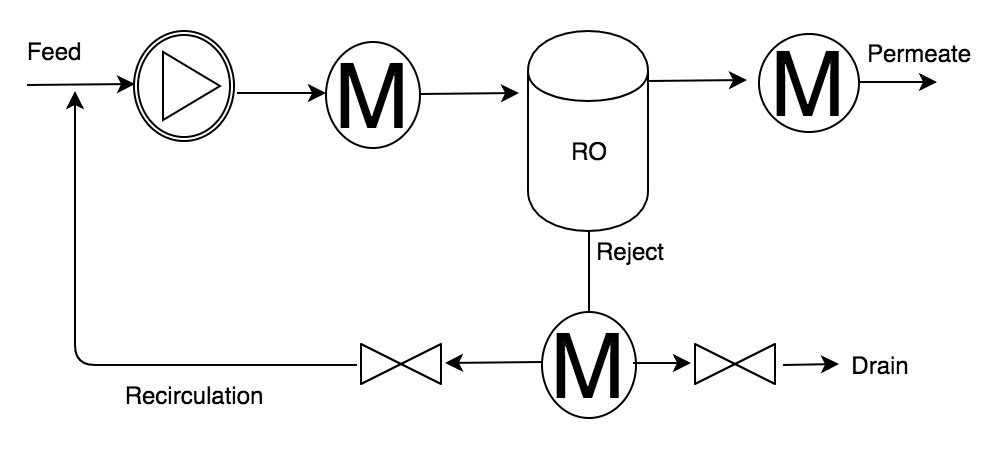
\includegraphics[width=0.4\textwidth]{MeasCurrSys}
    \caption{Current System, with measurement sensors}
    \label{fig:MeasCurrSys}
\end{figure}

\subsection{System 2  "Comparing system"}
A new, second system were built, according to Figure \ref{fig:MeasSys2} in order to do the tests for the modified system including two pumps. Same membrane, measurement senors were used.

\begin{figure}[h]
    \centering
    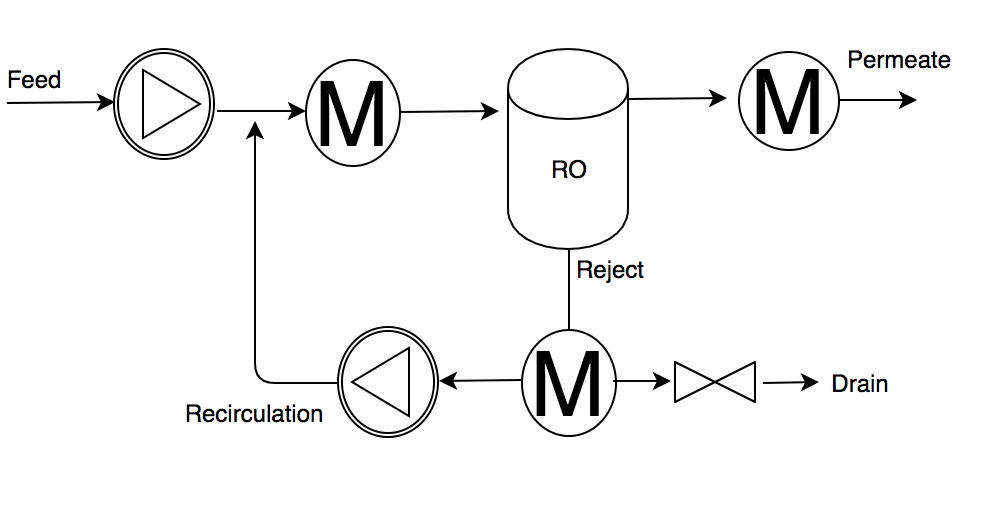
\includegraphics[width=0.4\textwidth]{MeasSys2}
    \caption{System 2, with measurement sensors}
    \label{fig:MeasSys2}
\end{figure}

\section{Connections} \label{Connections}

\begin{figure}[h]
    \centering
    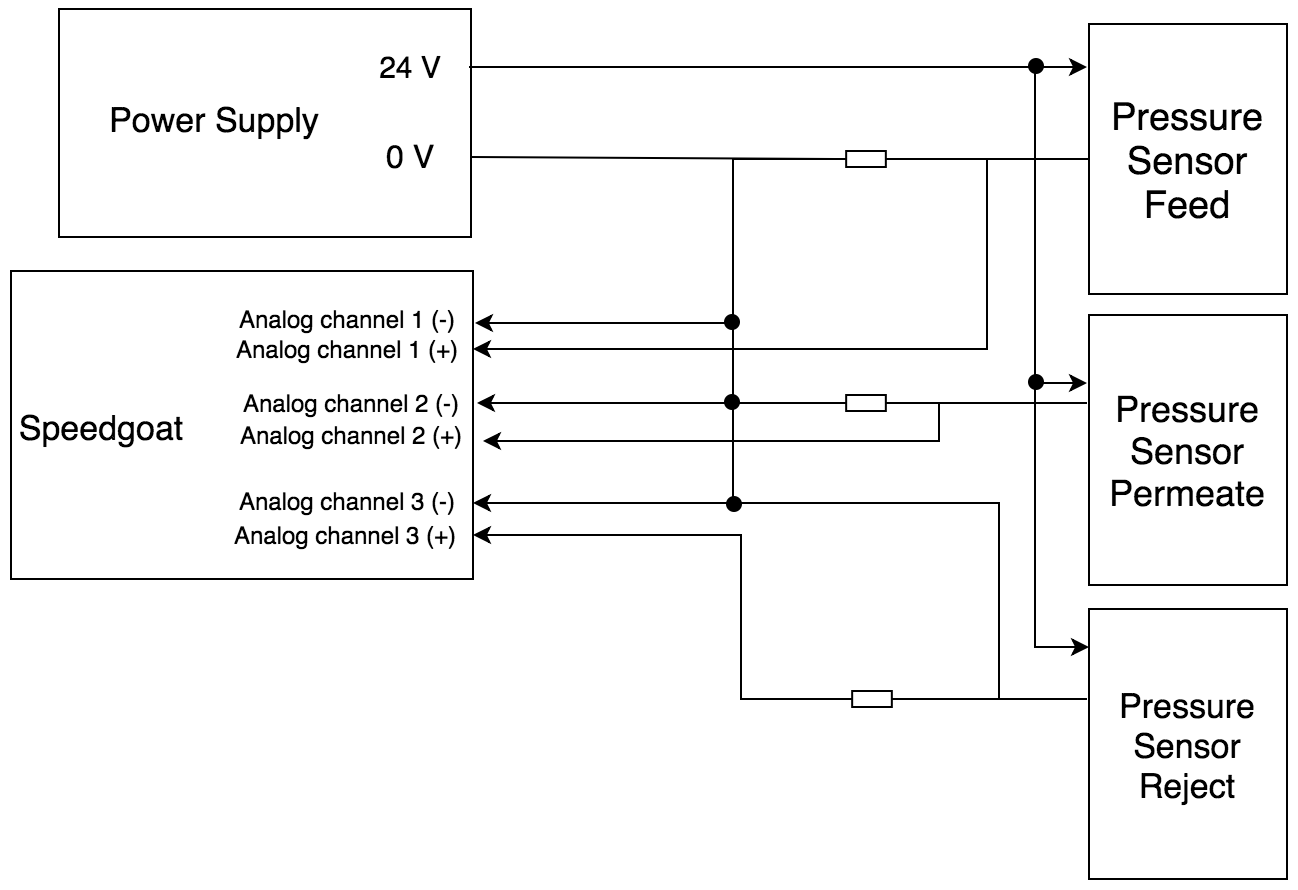
\includegraphics[width=0.7\textwidth]{PressConn}
    \caption{Connections Pressure sensors}
    \label{fig:PressConn}
\end{figure}

\begin{figure}[h]
    \centering
    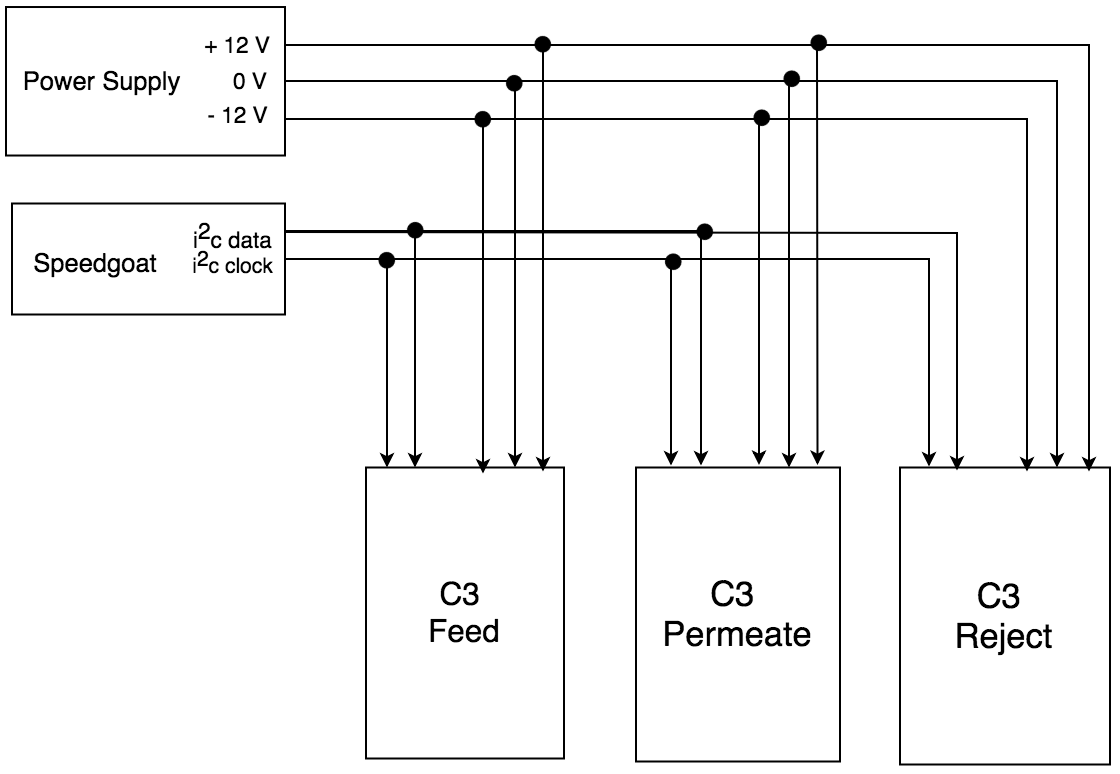
\includegraphics[width=0.7\textwidth]{C3Conn}
    \caption{Connections measurement blocks, C3}
    \label{fig:C3Conn}
\end{figure}

\begin{figure}[h]
    \centering
    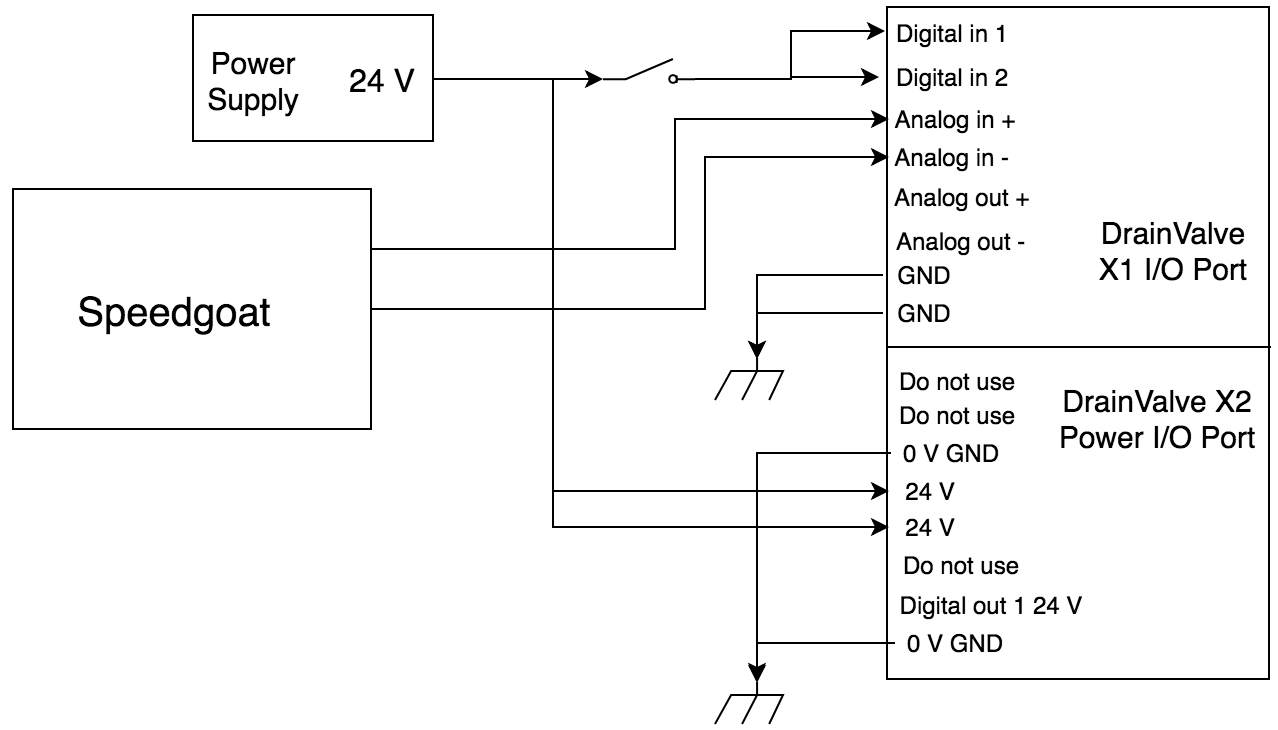
\includegraphics[width=0.7\textwidth]{ValveConn}
    \caption{Connections Drain Valve}
    \label{fig:ValveConn}
\end{figure}

\begin{figure}[h]
    \centering
    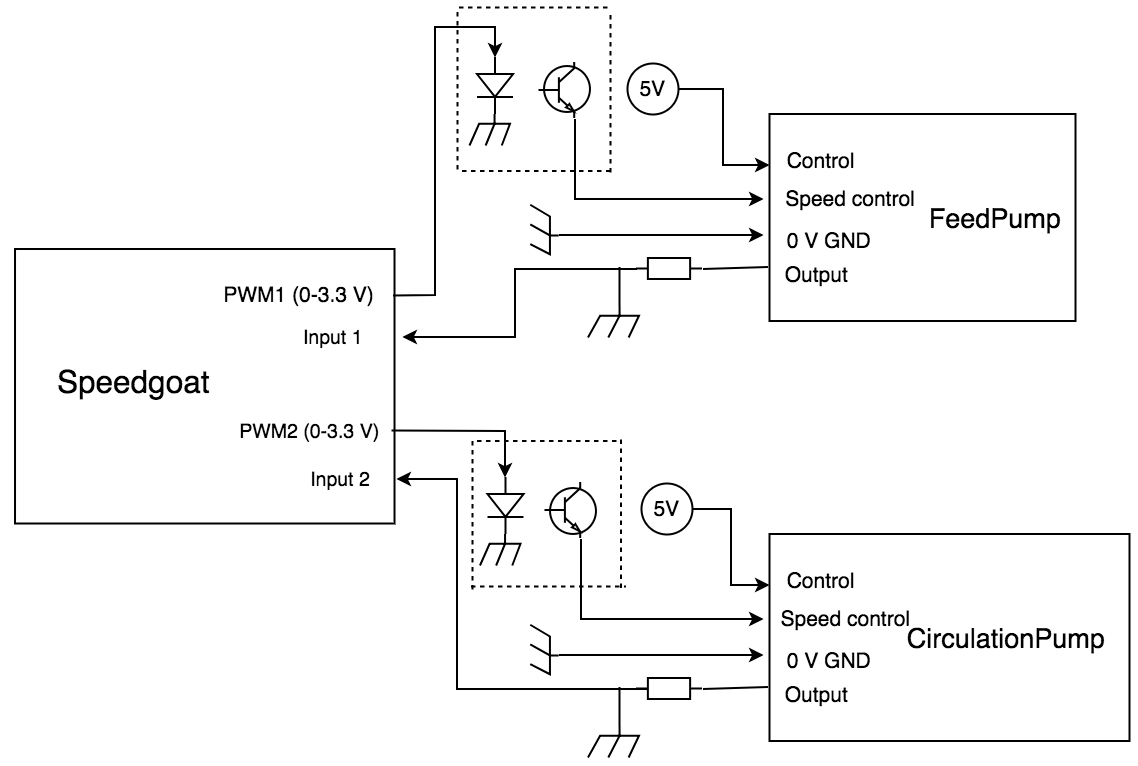
\includegraphics[width=0.7\textwidth]{PumpConn}
    \caption{Connections pumps}
    \label{fig:PumpConn}
\end{figure}


\section{Mapping}
In order to investigate the performance of the membrane pressure, flow, conductivity and temperature is to be measures. In the systems there are critical values of high pressure on feed side and reject side which makes it difficult to find measurement equipment that can handle both the high pressure and relatively low flows with no loss of pressure and required accuracy. Therefore some mapping of the flow were done and used. 

RPM - 

Flow - 



\section{Design of control algorithms}
Control algoritms were developed in Matlab Simulink for the updated system. 

\section{Control simulations}



\section{Improvements}

